\documentclass[a4paper, oneside]{memoir}
\usepackage[utf8]{inputenc}
\usepackage[T1]{fontenc}
\usepackage{pifont}
\usepackage{amssymb}
\usepackage{fourier}
\usepackage[dvipsnames]{xcolor}
\usepackage{tikz}
\usepackage{pdfpages}
\usepackage[sfdefault]{roboto}
\usepackage{color}

% Styles
\tikzstyle{teamshare} = [below, text width=5.4cm, inner sep = 0.5cm, text=white, align=center]
\tikzstyle{cardtext} = [below, text width=5.9cm, inner sep = 0.25cm, text centered]
\setlrmarginsandblock{0.9cm}{*}{1}
\setulmarginsandblock{1.49cm}{*}{1}
\checkandfixthelayout[nearest]
\pagestyle{empty}

% Define Commands
\newcommand{\condition}[1]{\textbf{#1}}
\newcommand{\character}[1]{\textbf{#1}}
\newdimen\titlespacing
\titlespacing=0.15cm

% Define Seperators
\newcommand{\seperator}[1]{\\ \vspace{\titlespacing} \hrulefill {} \tiny \bfseries #1 \normalfont \normalsize \hrulefill \\ \vspace{\titlespacing}}
\newcommand{\seperatoraction}{\seperator{POWER}}
\newcommand{\seperatordescription}{\seperator{DESCRIPTION}}
\newcommand{\seperatorcondition}{\seperator{CONDITION}}
\newcommand{\seperatorwin}{\seperator{HOW TO WIN}}
\newcommand{\redwinsection}{
	\seperatorwin
	\small You win if \character{President} gains the \condition{dead} condition due to the \character{Bomber} exploading.
}
\newcommand{\bluewinsection}{
	\seperatorwin
	\small You win if \character{President} does not gain the \condition{dead} condition due to the \character{Bomber} exploading.
}
\newcommand{\titlefrom}[1]{\\ \tiny > from #1 <\normalsize}

% Begin Document
\begin{document}
	
% New Page
\noindent 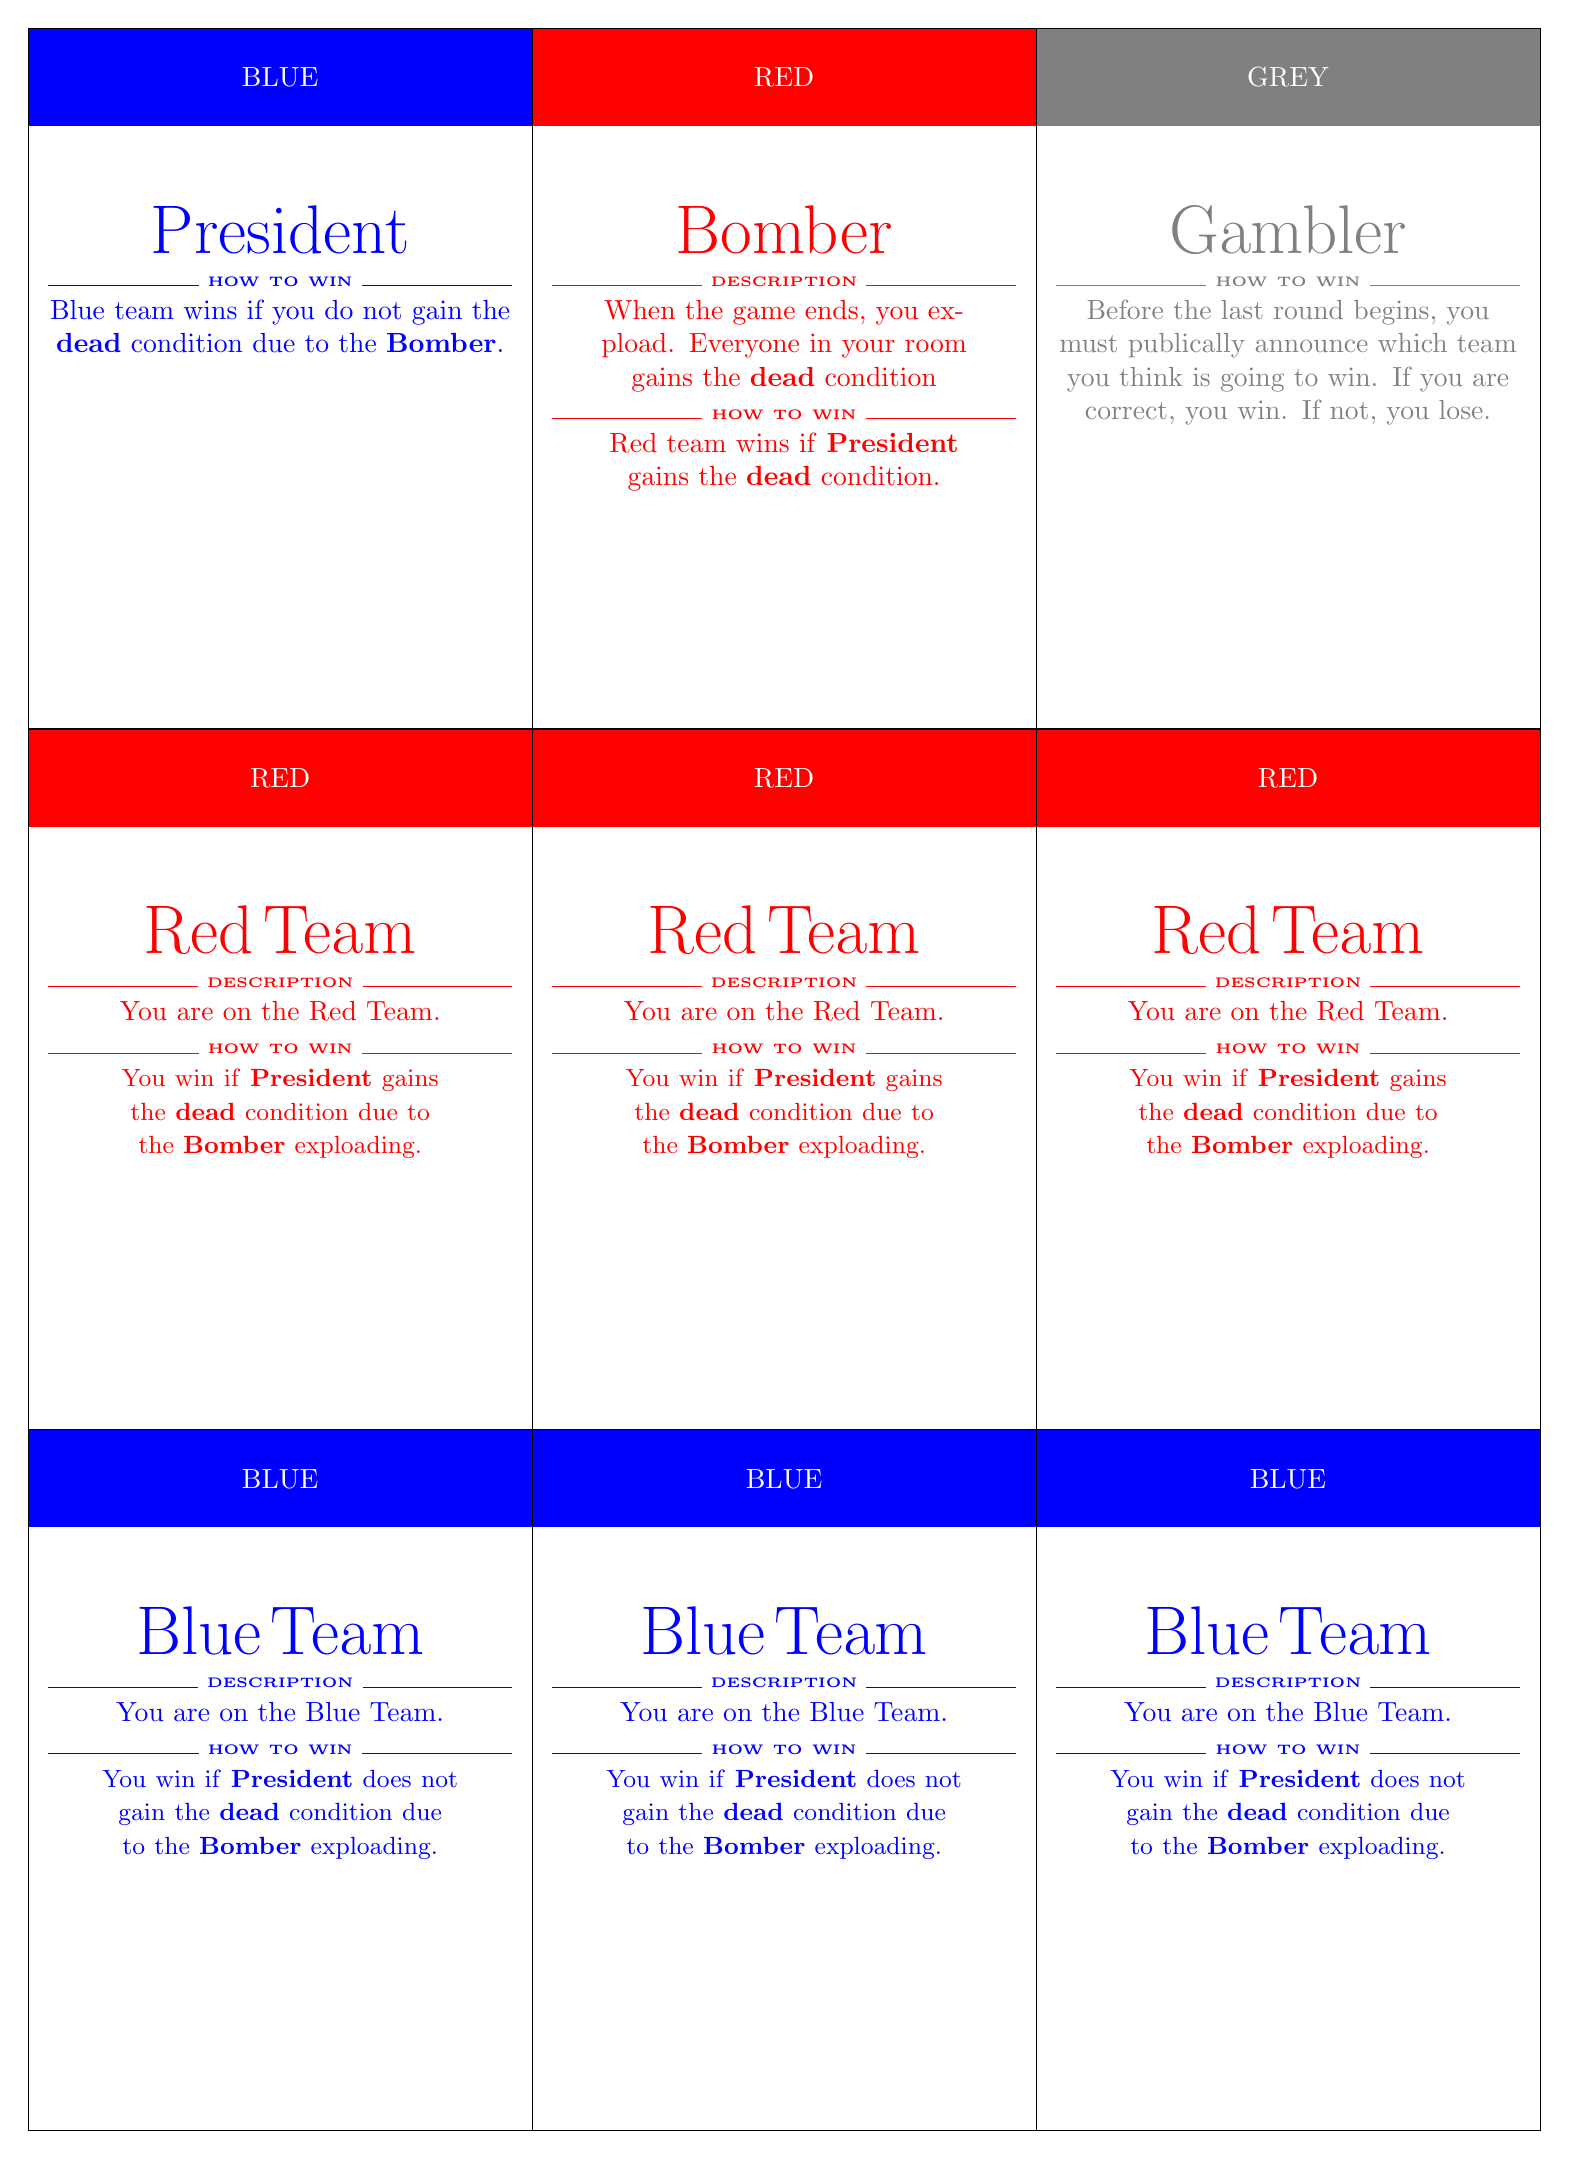
\begin{tikzpicture}[outer sep=0]

% PRESIDENT
\node[teamshare, fill=blue] (1) at (3.2,26.7) {\HUGE BLUE};
\node[cardtext, text=blue] at (3.2,24.7) {
	{\Huge President}
	\seperatorwin
	Blue team wins if you do not gain the \condition{dead} condition due to the \character{Bomber}.
	
};

% BOMBER
\node[teamshare, fill=red] at (9.6,26.7) {\HUGE RED};
\node[cardtext, text=red] at (9.6,24.7) {
	{\Huge Bomber}
	\seperatordescription
	When the game ends, you expload. Everyone in your room gains the \condition{dead} condition
	\seperatorwin
	Red team wins if \character{President} gains the \condition{dead} condition.
};

% GAMBLER
\node[teamshare, fill=gray] at (16,26.7) {\HUGE GREY};
\node[cardtext, text=gray] at (16,24.7) {
	{\Huge Gambler}
	\seperatorwin
	Before the last round begins, you must publically announce which team you think is going to win. If you are correct, you win. If not, you lose.
};

% RED TEAM MEMBER
\node[teamshare, fill=red] at (3.2,17.8) {\HUGE RED};
\node[cardtext, text=red] at (3.2,15.8) {
	{\Huge Red Team}
	\seperatordescription
	You are on the Red Team.
	\redwinsection
};

% RED TEAM MEMBER
\node[teamshare, fill=red] at (9.6,17.8) {\HUGE RED};
\node[cardtext, text=red] at (9.6,15.8) {
	{\Huge Red Team}
	\seperatordescription
	You are on the Red Team.
	\redwinsection
};

% RED TEAM MEMBER
\node[teamshare, fill=red] at (16,17.8) {\HUGE RED};
\node[cardtext, text=red] at (16,15.8) {
	{\Huge Red Team}
	\seperatordescription
	You are on the Red Team.
	\redwinsection
};

% BLUE TEAM MEMBER
\node[teamshare, fill=blue] at (3.2,8.9) {\HUGE BLUE};
\node[cardtext, text=blue] at (3.2,6.9) {
	{\Huge Blue Team}
	\seperatordescription
	You are on the Blue Team.
	\bluewinsection
};

% BLUE TEAM MEMBER
\node[teamshare, fill=blue] at (9.6,8.9) {\HUGE BLUE};
\node[cardtext, text=blue] at (9.6,6.9) {
	{\Huge Blue Team}
	\seperatordescription
	You are on the Blue Team.
	\bluewinsection
};

% BLUE TEAM MEMBER
\node[teamshare, fill=blue] at (16,8.9) {\HUGE BLUE};
\node[cardtext, text=blue] at (16,6.9) {
	{\Huge Blue Team}
	\seperatordescription
	You are on the Blue Team.
	\bluewinsection
};

\draw (0,0) -- (19.2,0);
\draw (0,8.9) -- (19.2,8.9);
\draw (0,17.8) -- (19.2,17.8);
\draw (0,26.7) -- (19.2,26.7);

\draw (0,0) -- (0,26.7);
\draw (6.4,0) -- (6.4,26.7);
\draw (12.8,0) -- (12.8,26.7);
\draw (19.2,0) -- (19.2,26.7);



\end{tikzpicture}

%Background is not my own. But courtesy of a user on BGG
\includepdf[pages={1}, angle=90]{cardsbackground.pdf}
\pagebreak

\noindent 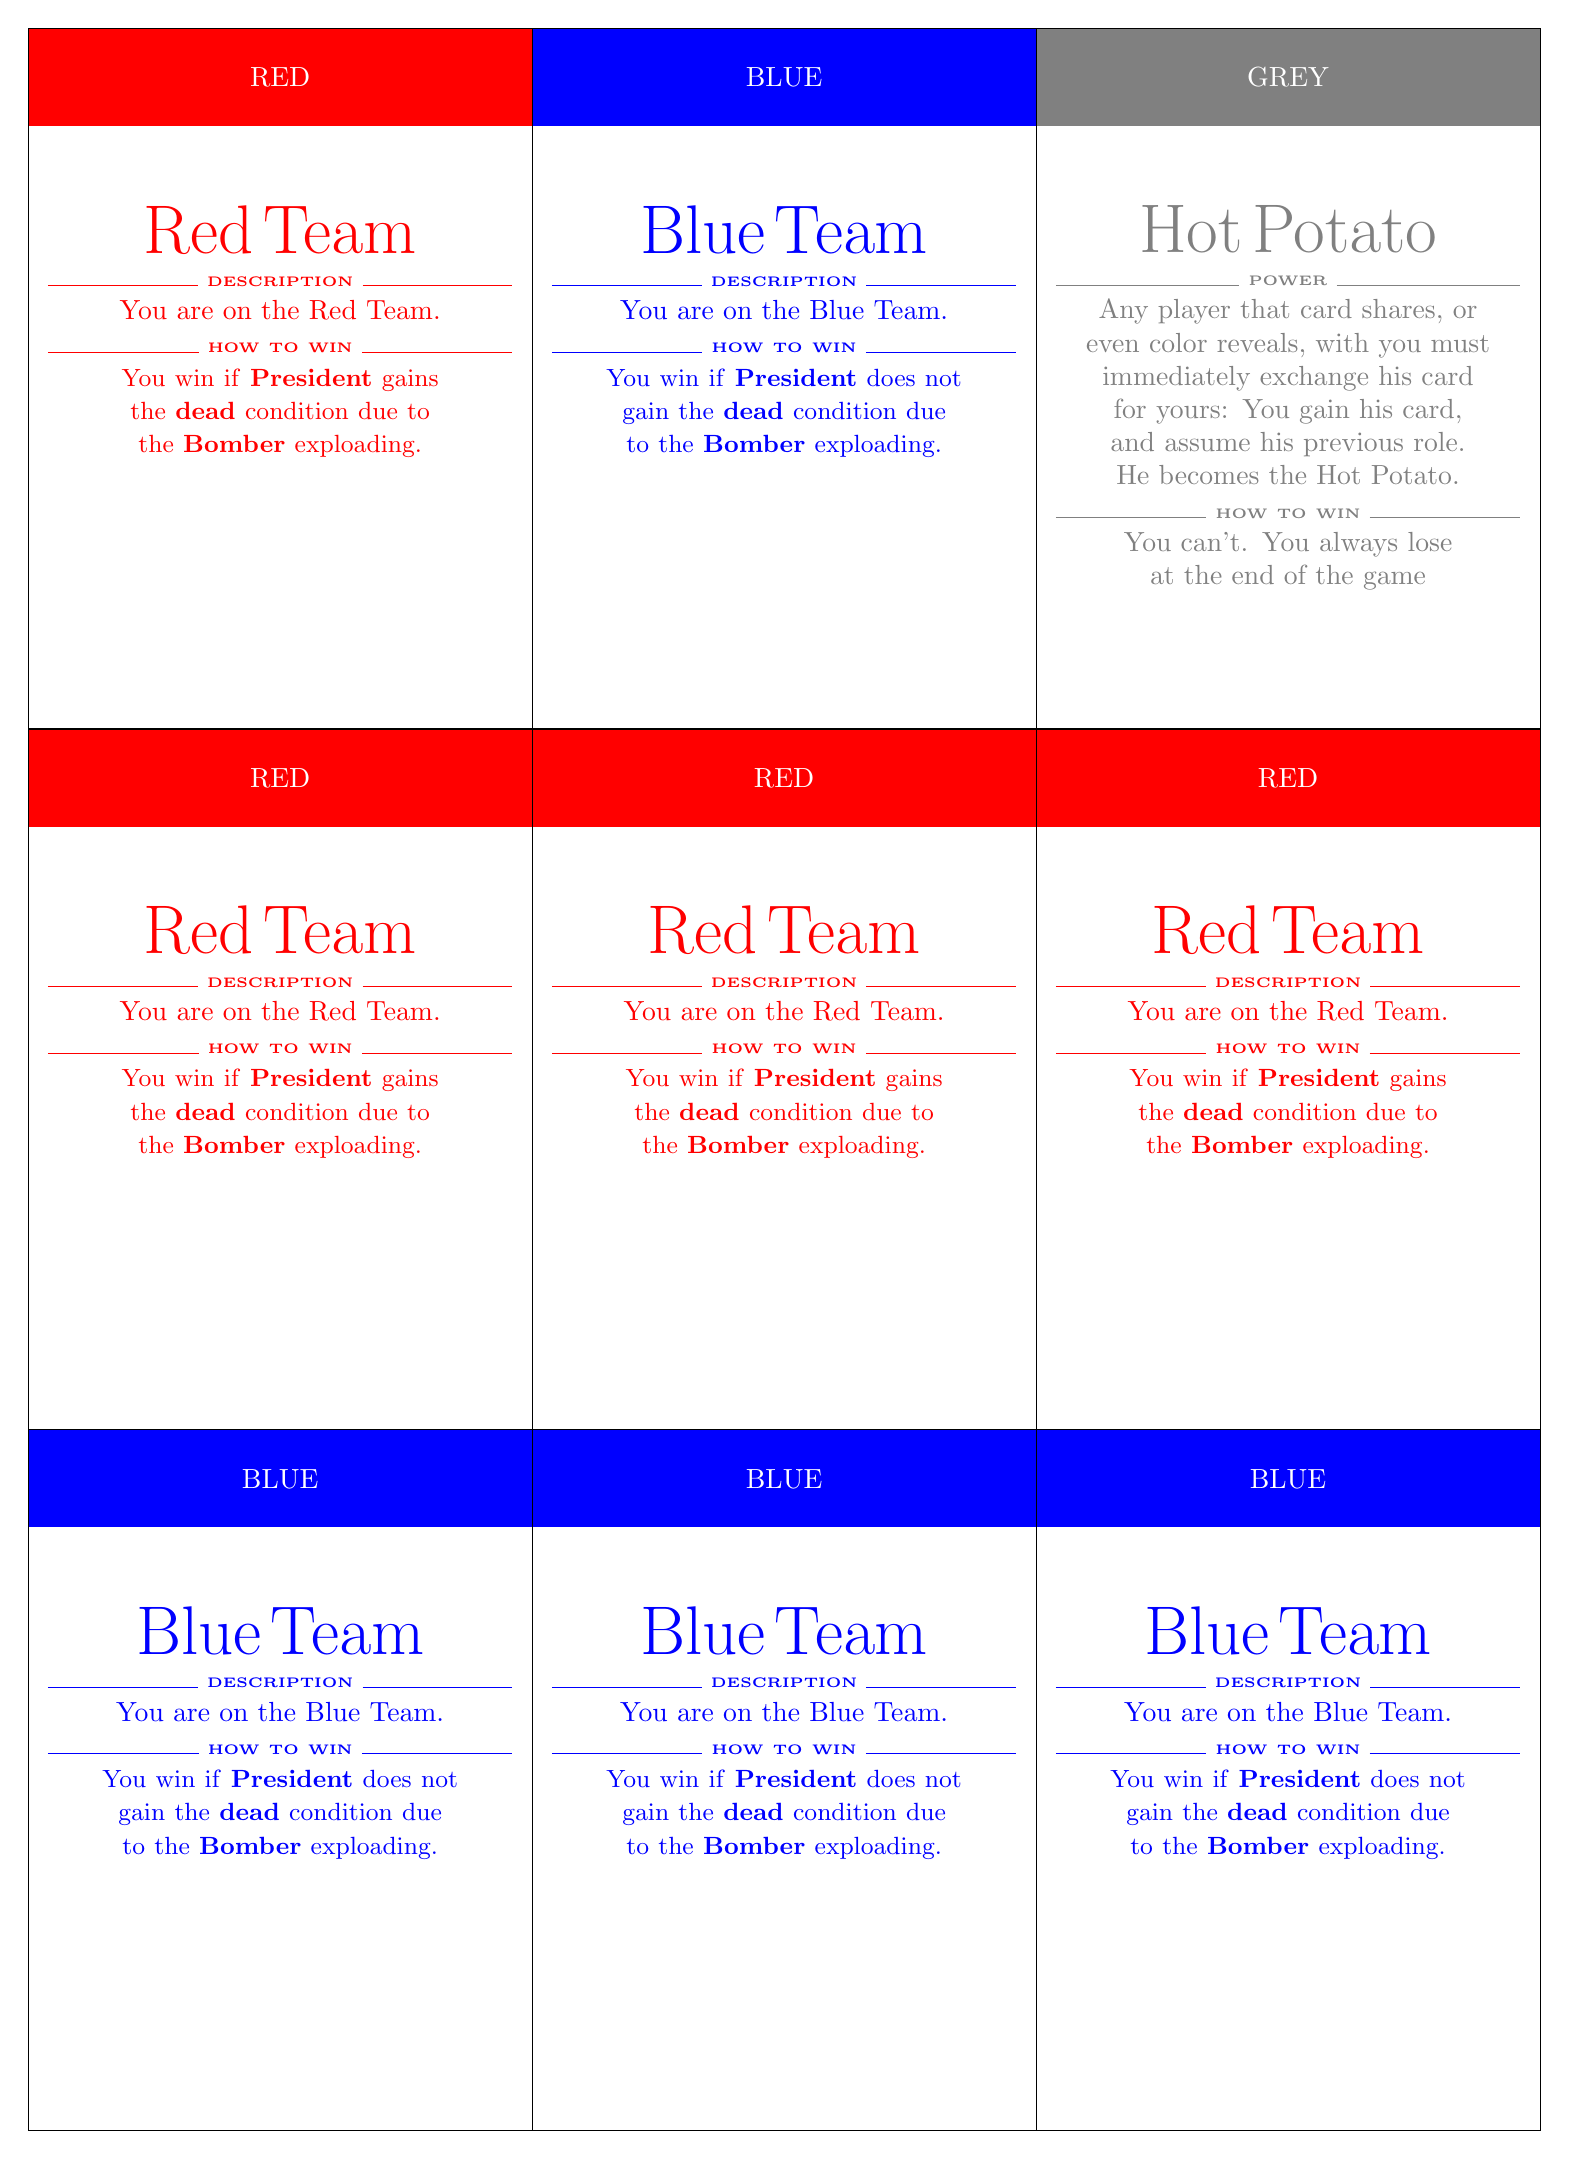
\begin{tikzpicture}[outer sep=0]

% RED TEAM MEMBER
\node[teamshare, fill=red] (1) at (3.2,26.7) {\HUGE RED};
\node[cardtext, text=red] at (3.2,24.7) {
	{\Huge Red Team}
	\seperatordescription
	You are on the Red Team.
	\redwinsection
};

% BLUE TEAM MEMBER
\node[teamshare, fill=blue] at (9.6,26.7) {\HUGE BLUE};
\node[cardtext, text=blue] at (9.6,24.7) {
	{\Huge Blue Team}
	\seperatordescription
	You are on the Blue Team.
	\bluewinsection
};

% HOT POTATO
\node[teamshare, fill=gray] at (16,26.7) {\HUGE GREY};
\node[cardtext, text=gray] at (16,24.7) {
	{\Huge Hot Potato}
	\seperatoraction
	Any player that card shares, or even color reveals, with you must immediately exchange his card for yours: You gain his card, and assume his previous role. He becomes the Hot Potato.
	\seperatorwin
	You can't. You always lose at the end of the game	
};

% RED TEAM MEMBER
\node[teamshare, fill=red] at (3.2,17.8) {\HUGE RED};
\node[cardtext, text=red] at (3.2,15.8) {
	{\Huge Red Team}
	\seperatordescription
	You are on the Red Team.
	\redwinsection
};

% RED TEAM MEMBER
\node[teamshare, fill=red] at (9.6,17.8) {\HUGE RED};
\node[cardtext, text=red] at (9.6,15.8) {
	{\Huge Red Team}
	\seperatordescription
	You are on the Red Team.
	\redwinsection
};

% RED TEAM MEMBER
\node[teamshare, fill=red] at (16,17.8) {\HUGE RED};
\node[cardtext, text=red] at (16,15.8) {
	{\Huge Red Team}
	\seperatordescription
	You are on the Red Team.
	\redwinsection
};

% BLUE TEAM MEMBER
\node[teamshare, fill=blue] at (3.2,8.9) {\HUGE BLUE};
\node[cardtext, text=blue] at (3.2,6.9) {
	{\Huge Blue Team}
	\seperatordescription
	You are on the Blue Team.
	\bluewinsection
};

% BLUE TEAM MEMBER
\node[teamshare, fill=blue] at (9.6,8.9) {\HUGE BLUE};
\node[cardtext, text=blue] at (9.6,6.9) {
	{\Huge Blue Team}
	\seperatordescription
	You are on the Blue Team.
	\bluewinsection
};

% BLUE TEAM MEMBER
\node[teamshare, fill=blue] at (16,8.9) {\HUGE BLUE};
\node[cardtext, text=blue] at (16,6.9) {
	{\Huge Blue Team}
	\seperatordescription
	You are on the Blue Team.
	\bluewinsection
};

\draw (0,0) -- (19.2,0);
\draw (0,8.9) -- (19.2,8.9);
\draw (0,17.8) -- (19.2,17.8);
\draw (0,26.7) -- (19.2,26.7);
\draw (0,0) -- (0,26.7);
\draw (6.4,0) -- (6.4,26.7);
\draw (12.8,0) -- (12.8,26.7);
\draw (19.2,0) -- (19.2,26.7);

\end{tikzpicture}

\includepdf[pages={1}, angle=90]{cardsbackground.pdf}

\end{document}